\documentclass[a4paper,10pt]{article}
\usepackage[utf8]{inputenc}
\usepackage{polski}
\usepackage{graphicx}
\usepackage{listings}
\usepackage{amsmath,amsfonts,amsthm} % Math packages
\usepackage[usenames,dvipsnames]{color}
\addtolength{\hoffset}{-1cm}
\addtolength{\voffset}{-2cm}
\addtolength{\textwidth}{2cm}
\addtolength{\textheight}{3cm}

\title{Informatyczne Systemy Sterowania \\ \large Ćwiczenie 1: Podstawy tworzenia opisów i modelowania obiektów sterowania}

\author{Krzysztof Przybylski 239266}

\lstset{
    language=Matlab,
    basicstyle=\scriptsize,
    aboveskip={1.5\baselineskip},
    columns=fixed,
    showstringspaces=false,
    extendedchars=true,
    breaklines=true,
    tabsize=4,
    prebreak = \raisebox{0ex}[0ex][0ex]{\ensuremath{\hookleftarrow}},
    frame=single,
    showtabs=false,
    showspaces=false,
    showstringspaces=false,
    identifierstyle=\ttfamily,
    keywordstyle=\color[rgb]{0,0,1},
    commentstyle=\color[rgb]{0.133,0.545,0.133},
    stringstyle=\color[rgb]{0.627,0.126,0.941},
    numbers=left,
    numberstyle=\tiny,
    stepnumber=1,
    numbersep=5pt,
    captionpos=b,
    escapeinside={\%*}{*)}
}



\begin{document}
\maketitle

\section{Wstęp}\label{sec:wstęp}
%TODO skopiowane z listy (trzeba to przerobić)
Tworzenie opisów (modeli) matematycznych obiektów sterowania, a także wykorzystanie tych opisów do badania i analizy (modelowania) obiektów – są istotnymi czynnościami w trakcie projektowania informatycznych systemów sterowania. Do realizacji tych czynności w praktyce inżynierskiej powszechnie stosuje się narzędzie informatyczne Matlab wraz ze specjalistycznym oprogramowaniem dodatkowym (tzw. toolbox’y) oraz nakładką Simulink.

\section{Zadanie 1 \textit{\small Tworzenie modeli matematycznych}}\label{sec:zad1}

\begin{itemize}
	
\item Człon proporcjonalny
\begin{itemize}
	\item Równanie różniczkowe
	\begin{eqnarray} 
	 y(t) = k\textsubscript p * u(t)
	\end{eqnarray}
	\item Transmitancja	
	\begin{eqnarray}
	G(s) = k
	\end{eqnarray}
	\item Wektor stanu i opis w przestrzeni stanu
	\newline Nie istnieje wektor stanu i opis w przestrzeni stanu - zerowy rząd równania różniczkowego.
\end{itemize}
	
	
\item Człon różniczkujący
	\begin{itemize}
		\item Równanie różniczkowe
		\begin{eqnarray}
 		y(t) = k * \dot{u}(t)
		\end{eqnarray}
		\item Transmitancja
		\begin{eqnarray}
		G(s) = k*s
		\end{eqnarray}
		\item Wektor stanu i opis w przestrzeni stanu
		\newline Nie istnieje wektor stanu i opis w przestrzeni stanu - zerowy rząd równania różniczkowego.
	\end{itemize}
	
	
\item Człon całkujący

\begin{itemize}
	\item Równanie różniczkowe
	\begin{eqnarray} 
	y(t) = k\textsubscript i * \int_{0}^{t} u(t)dt
	\end{eqnarray}	
	\item Transmitancja	
	\begin{eqnarray}
	G(s) = \frac{k}{s}
	\end{eqnarray}

	\item Wektor stanu i opis w przestrzeni stanu

Wykorzystując wektor stanu równy:
\begin{equation}
x(t) = [y(t)]
\end{equation}
oraz powyższe równanie różniczkowe, można wyznaczyć opis przestrzeni stanu:
\begin{equation}
\begin{split}
&y(t) = k\textsubscript i * \int_{0}^{t} u(t)dt \iff \dot{y}(t) = k\textsubscript i u(t)\\
&\dot{x}(t) = \dot{y}(t)
\end{split}
\end{equation}
Z ogólnego równania stanu:
\begin{equation}
\begin{split}
\dot{x}(t) = Ax(t) + Bu(t)\\
y(t) = Cx(t) + Du(t)
\end{split}
\end{equation}
oraz opisu przestrzeni:
\begin{equation}
\begin{split}
&\dot{x}(t) = k * u(t)\\
&y(t) = x(t)
\end{split}
\end{equation}
wyznaczam macierze:
\begin{equation}
A =
\begin{bmatrix}
0
\end{bmatrix}
B =
\begin{bmatrix}
k
\end{bmatrix}
C =
\begin{bmatrix}
1
\end{bmatrix}
D =
\begin{bmatrix}
0
\end{bmatrix}
\end{equation}
\item Opis przy pomocy Matlaba
\newline Aby uzyskać opis przy pomocy Matlaba wykorzystałem funkcję zmiany transformaty do równania przestrzeni stanu
\begin{equation}
[A,B,C,D]
= tf2ss(b,a)
\end{equation}
\newline Dla $k=1$, $T=2$

Otrzymałem wynik:
$A = \left[ \begin{array}{ll} -0.5 & 0\\ 1 & 0 \end{array} \right], B = \left[ \begin{array}{l} 1\\ 0 \end{array} \right], C = \left[ \begin{array}{ll} 0 & 0.5 \end{array} \right]$
\newline \newline Parametry zwrócone przez Matlaba różnią się od obliczonych przez nas prawdopodobnie dlatego, że Matlab przyjął inny wektor x(t) na samym początku. Jednak oba opisy są równoważne, ponieważ można przedstawić je w taki sposób:
\begin{eqnarray}
\nonumber \left\{ \begin{array}{l}
\dot{x_{1}}(t) = -0.5x_{1}(t) + u(t)\\
\dot{x_{2}}(t) = x_{1}\\
y(t) = 0.5x(t)
\end{array} \right. \\
\nonumber \ddot{y}(t) = 0.5\ddot{x_{2}}(t)\\
\nonumber \ddot{y}(t) = 0.5\dot{x_{1}}(t)\\
\nonumber \ddot{y}(t) = -0.25x_{1}(t) + 0.5u(t)\\
\nonumber \ddot{y}(t) = -0,5\dot{y}(t) + 0.5u(t)\\
2\ddot{y}(t) + \dot{y}(t) = u(t)
\end{eqnarray}
Po porównaniu wyniku przekształceń widzimy, że $k=1$, $T=2$, czyli tak jak założyliśmy.	
\end{itemize}
	
\item Człon inercyjny I rzędu

\begin{itemize}
	\item Równanie różniczkowe
	\begin{eqnarray}
	T\dot{y}(t)+y(t) = k\textsubscript I *u(t)
	\end{eqnarray}
	
\item Transmitancja	
	\begin{eqnarray}
		G(s) = \frac{k}{T*s+1}
	\end{eqnarray}

\item Wektor stanu i opis w przestrzeni stanu
\newline Przyjmując wektor stanu równy: \[ x(t) = [y(t)] \]
oraz powyższe równanie różniczkowe, można wyznaczyć opis przestrzeni stanu:
\begin{equation}
\begin{split}
&\dot{y}(t) = -\frac{x(t)}{T} + \frac{k u(t)}{T}\\
&\dot{x}(t) = \dot{y}(t)\\
&\dot{x}(t) = -\frac{x(t)}{T} + \frac{k u(t)}{T}\\
&y(t) = x(t)
\end{split}
\end{equation}
wyznaczyć można następujące macierze:
\begin{equation}
A =
\begin{bmatrix}
-\frac{1}{T}
\end{bmatrix}\\
B =
\begin{bmatrix}
\frac{k}{T}
\end{bmatrix}\\
C =
\begin{bmatrix}
1
\end{bmatrix}\\
D =
\begin{bmatrix}
0
\end{bmatrix}
\end{equation}
\item Opis przy pomocy Matlaba
\newline W celu uzyskania opisu przy pomocy Matlaba wykorzystam funkcję
\begin{equation}
[A,B,C,D]
= tf2ss(b,a)
\end{equation}
Ustalam wartość k = 8 i T = 2.
Mając te dane wyliczam:
\begin{equation}
\begin{split}
&[A, B, C, D]
= tf2ss(8, \begin{bmatrix}
2 && 1
\end{bmatrix})\\
&A =
\begin{bmatrix}
-\frac{1}{2}
\end{bmatrix}\\
&B =
\begin{bmatrix}
1
\end{bmatrix}\\
&C =
\begin{bmatrix}
4
\end{bmatrix}\\
&D =
\begin{bmatrix}
0
\end{bmatrix}
\end{split}
\end{equation}

Możemy udowodnić równoważność wyników z Matlaba oraz wcześniej wyliczonych.

Wykorzystuję funkcję ss2tf.
Otrzymane wyniki wyglądają następująco:
\begin{equation}
\begin{split}
&[b,a]
= ss2tf(A, B, C, D)\\
&b = \begin{bmatrix}
0 && 4
\end{bmatrix}\\
&a = \begin{bmatrix}
1 && 1/2
\end{bmatrix}
\end{split}
\end{equation}
Korzystając z wyżej wymienionych parametrów otrzymuję następującą transmitancję operatorową:
\begin{equation}
G(s) = \frac{4}{s +\frac{1}{2}} = \frac{8}{2s+1}
\end{equation}

Zarówno ręcznie wyliczone opisy przestrzeni stanu jak i te wyliczone przez Matlaba wskazują na ten sam człon.

\end{itemize}

\item Człon oscylacyjny
\begin{itemize}
		\item Równanie różniczkowe
	\begin{eqnarray} 
	 T\textsubscript n ^2 \ddot{y}(t) + 2\zeta T\textsubscript n \dot{y}(t) + y(t) = ku
	\end{eqnarray}	
	\item Transmitancja	
	\begin{eqnarray}
	 G(s) = \frac{k}{T\textsubscript n ^2s^2 + 2\zeta T\textsubscript n s + 1}
	\end{eqnarray}
	
	\item Wektor stanu i opis w przestrzeni stanu
	\newline Przyjmując wektor stanu równy:
	\begin{equation}
	x =\begin{bmatrix}
	y(t) \\
	\dot{y}(t)
	\end{bmatrix}
	\end{equation}
	oraz wyżej wymienione równanie różniczkowe, można wyznaczyć opis przestrzeni stanu:
	\begin{equation}
	\begin{split}
	&x\textsubscript 1 (t) = y(t)\\
	&x\textsubscript 2 (t) = \dot{y}(t)\\
	&T\textsubscript n ^2 \dot{x}\textsubscript 2 (t) + 2 \zeta T\textsubscript n x\textsubscript 2 (t) + x\textsubscript 1 (t) = ku\\
	&\dot{x}\textsubscript 2 (t) = -\frac{2\zeta T\textsubscript n}{T\textsubscript n ^2} x\textsubscript 2 (t) - \frac{1}{T\textsubscript n ^2} x\textsubscript 1 (t) + \frac{k}{T\textsubscript n ^2} u\\
	\end{split}
	\end{equation}
	oraz macierze:
	\begin{equation}
	A =
	\begin{bmatrix}
	0 && 1 \\
	-\frac{1}{T\textsubscript n ^2} && -\frac{2\zeta T\textsubscript n }{T\textsubscript n ^2}
	\end{bmatrix}\\
	B =
	\begin{bmatrix}
	0 \\
	\frac{k}{{T\textsubscript n} ^2}
	\end{bmatrix}\\
	C =
	\begin{bmatrix}
	1
	\end{bmatrix}\\
	D =
	\begin{bmatrix}
	0
	\end{bmatrix}
	\end{equation}
	\item Opis przy pomocy Matlaba
	W celu uzyskania opisu przy pomocy Matlaba wykorzystam funkcję
	\begin{equation}
	[A,B,C,D]
	= tf2ss(b,a)
	\end{equation}
	oraz przyjmę następujące wartości:
	\begin{equation}
	\begin{split}
	&T\textsubscript n = 3\\
	&k = 5\\
	&\zeta = 2
	\end{split}
	\end{equation}
	Wtedy macierze będą wyglądały następująco:
	\begin{equation}
	\begin{split}
	&[A, B, C, D]
	= tf2ss(5, \begin{bmatrix}
	9 && 12 && 1
	\end{bmatrix})\\
	&A =
	\begin{bmatrix}
	-1\frac{1}{3} && -\frac{1}{9}\\
	1 && 0
	\end{bmatrix}\\
	&B =
	\begin{bmatrix}
	1\\
	0
	\end{bmatrix}\\
	&C =
	\begin{bmatrix}
	0 && \frac{5}{9}
	\end{bmatrix}\\
	&D =
	\begin{bmatrix}
	0
	\end{bmatrix}
	\end{split}
	\end{equation}
	\newline Dowód równoważności wyników wyliczonych oraz tych z Matlaba.
	\newline\newline Macierze wyliczone ręcznie oraz otrzymane przy pomocy programu Matlab wydają się bardzo różne.
	Macierz A przeszła transformacją, tak samo jak macierz B. Macierz C ma więcej kolumn.
	Macierze D są takie same.\\
	Wykorzystuję powtórnie funkcję ss2tf.
	Otrzymane wyniki prezentują się następująco:
	\begin{equation}
	\begin{split}
		&[b,a]
		= ss2tf(A, B, C, D)\\
		&b = \begin{bmatrix}
		0 && 0 && \frac{5}{9}
		\end{bmatrix}\\
		&a = \begin{bmatrix}
		1 && 1\frac{1}{3} && \frac{1}{9}
		\end{bmatrix}
	\end{split}
	\end{equation}
	Korzystając z wyżej wymienionych parametrów otrzymamy następującą transmitancję operatorową:
	\begin{equation}
	G(s) = \frac{5}{9s^2 + 12s + 1} = \frac{\frac{5}{9}}{1s^2 + 1\frac{1}{3}s + \frac{1}{9}}
	\end{equation}
	Z czego wynika, że obydwa zapisy przestrzeni stanu są poprawne.
\end{itemize}

\item Człon opóźniający
\begin{itemize}
	\item Równanie różniczkowe
	\begin{equation}
	y(t) = k\textsubscript o u(t-T\textsubscript 0)
	\end{equation}
	\item Transmitancja
	\begin{equation}
	G(s) = ke^{-sT\textsubscript 0}
	\end{equation}
	\item Wektor stanu i opis w przestrzeni stanu
	
	Nie istnieje wektor stanu i opis w przestrzeni stanu - zerowy rząd równania różniczkowego.
\end{itemize}
\end{itemize}

\section{Zadanie 2 \textit{\small Wyznaczanie charakterystyk czasowych}}\label{sec:zad2}

\begin{itemize}
\item Człon proporcjonalny

	Przyjąłem k = 8
	\begin{center}
		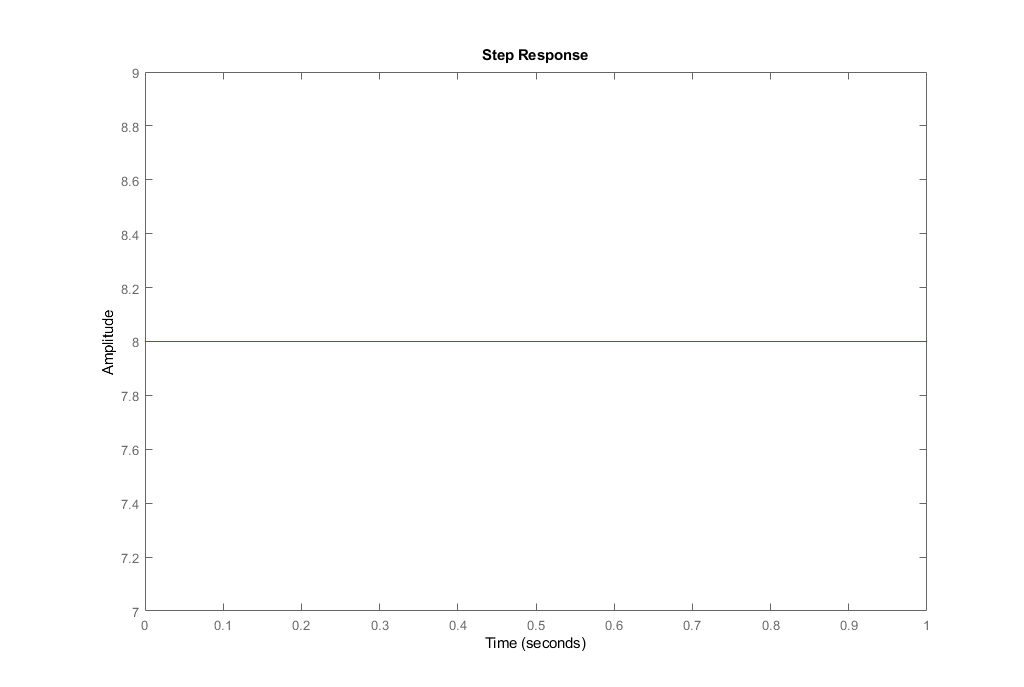
\includegraphics[width=15cm]{prop_step.png}
		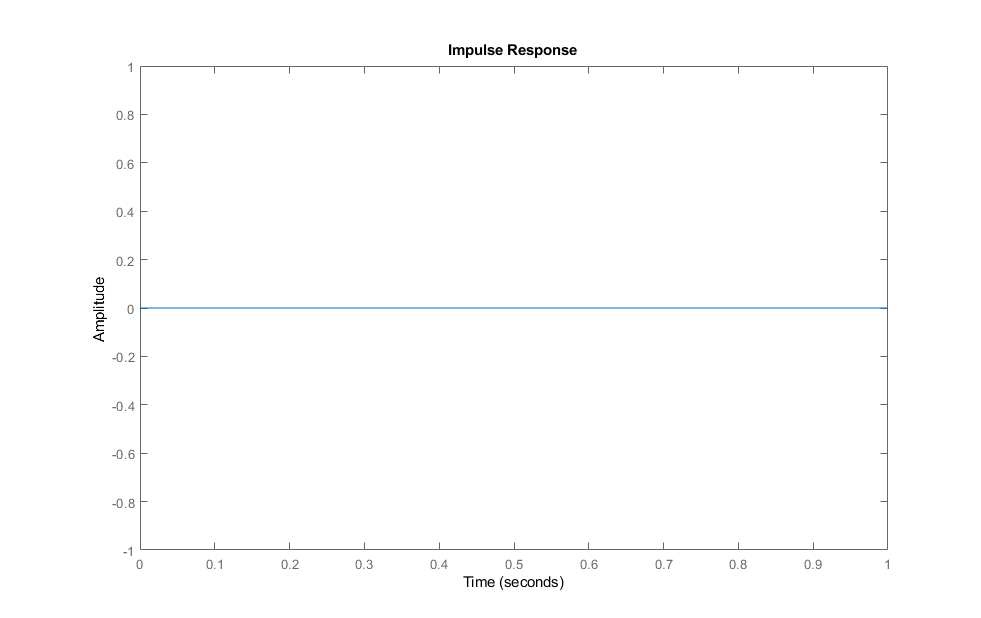
\includegraphics[width=15cm]{prop_impulse.png}
	\end{center}
	
	
\item Człon całkujący

	Przyjąłem k = 8
	
	\begin{center}
		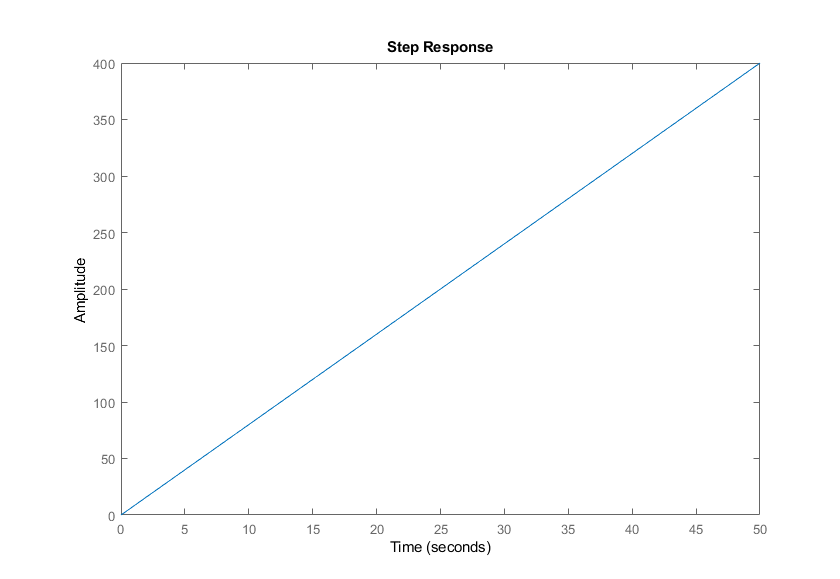
\includegraphics[width=15cm]{cal_step.png}
		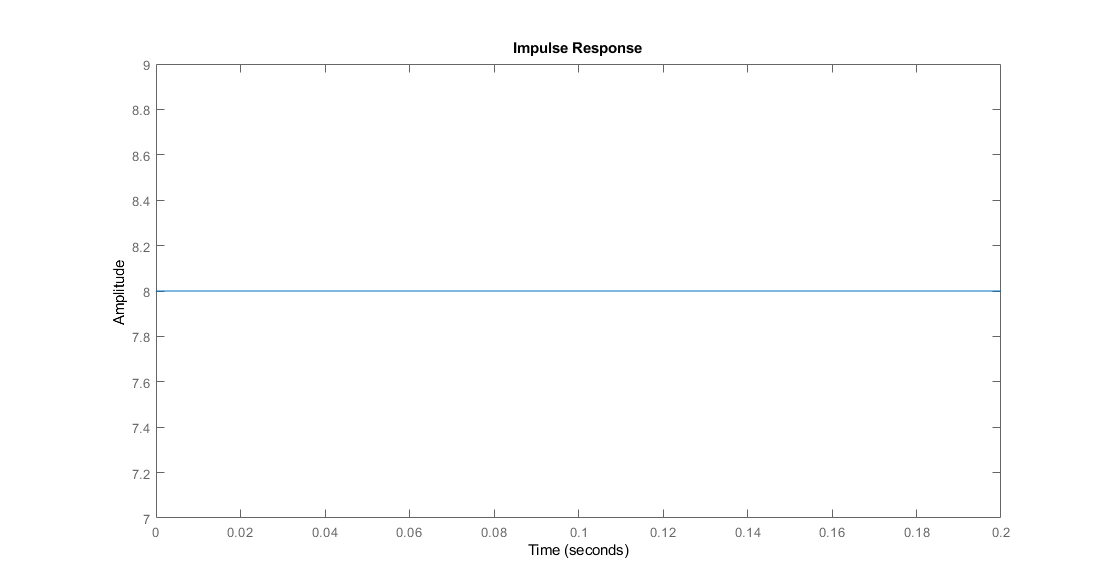
\includegraphics[width=15cm]{cal_impulse.png}
	\end{center}
	
\item Człon inercyjny I rzędu

	Przyjąłem k = 8 oraz T = 6
	
	\begin{center}
		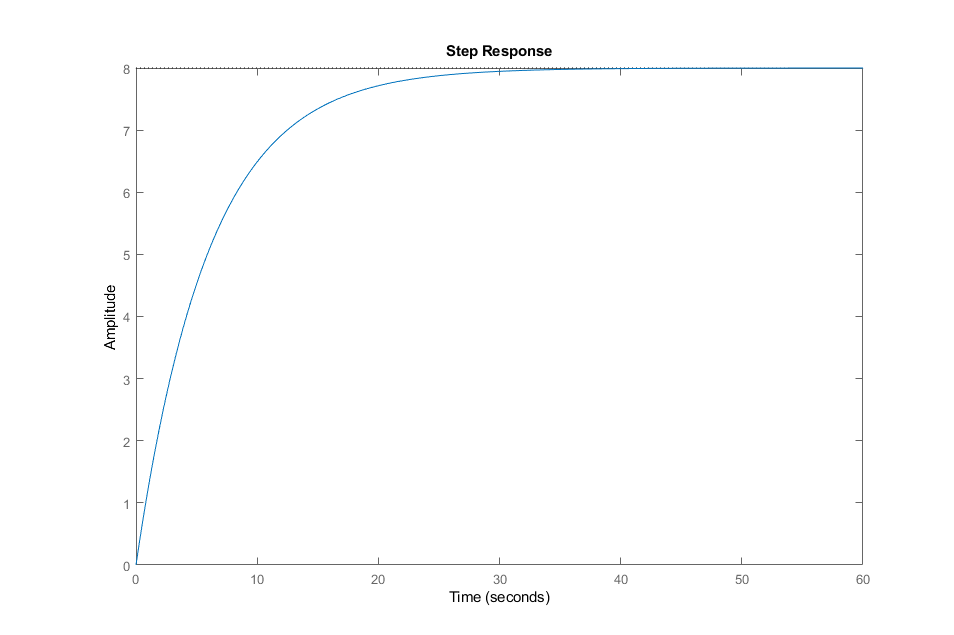
\includegraphics[width=15cm]{iner1_step.png}
		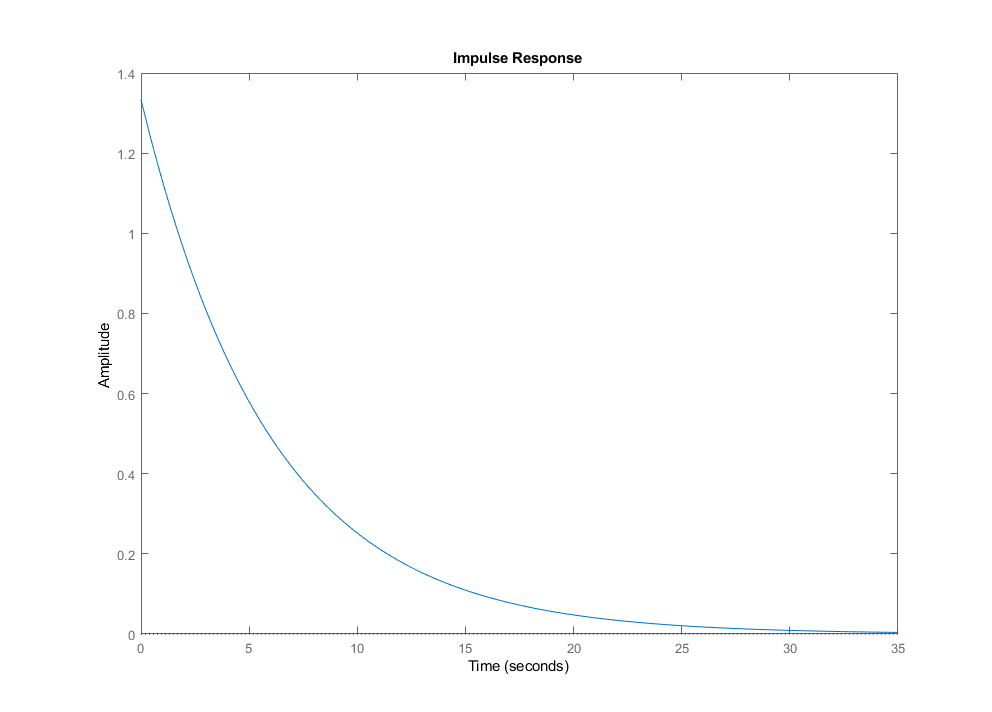
\includegraphics[width=15cm]{iner1_impulse.png}
	\end{center}
	
\item Człon oscylacyjny
	 
	 Przyjąłem:
	\begin{equation}
 k = 8, T\textsubscript{n} = 6, \zeta = 2
	\end{equation}

	\begin{center}
		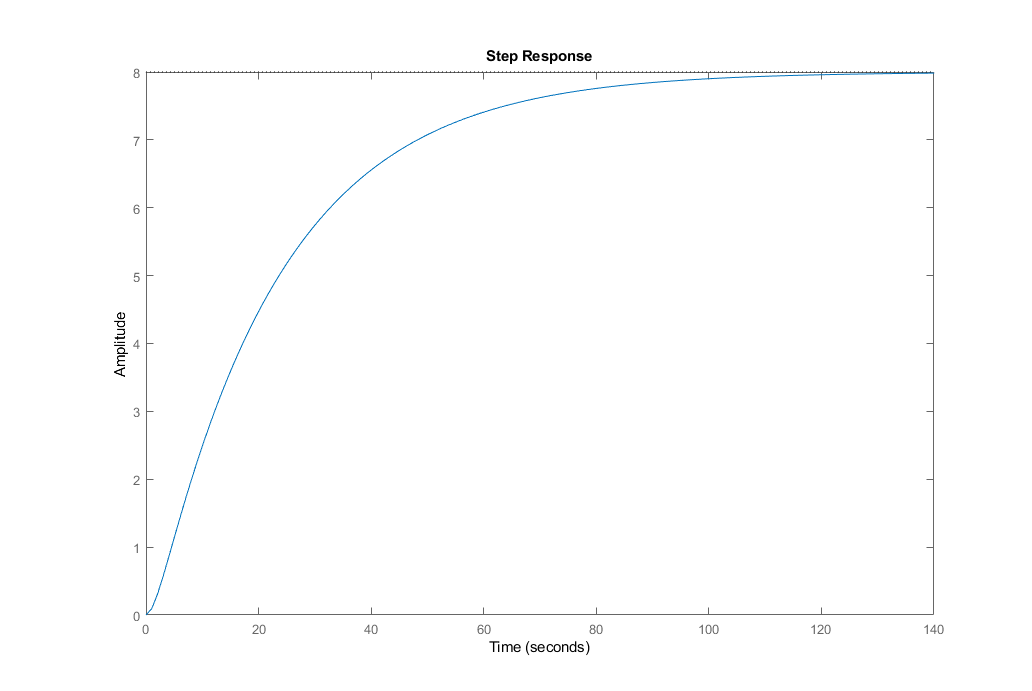
\includegraphics[width=15cm]{osc_step.png}
		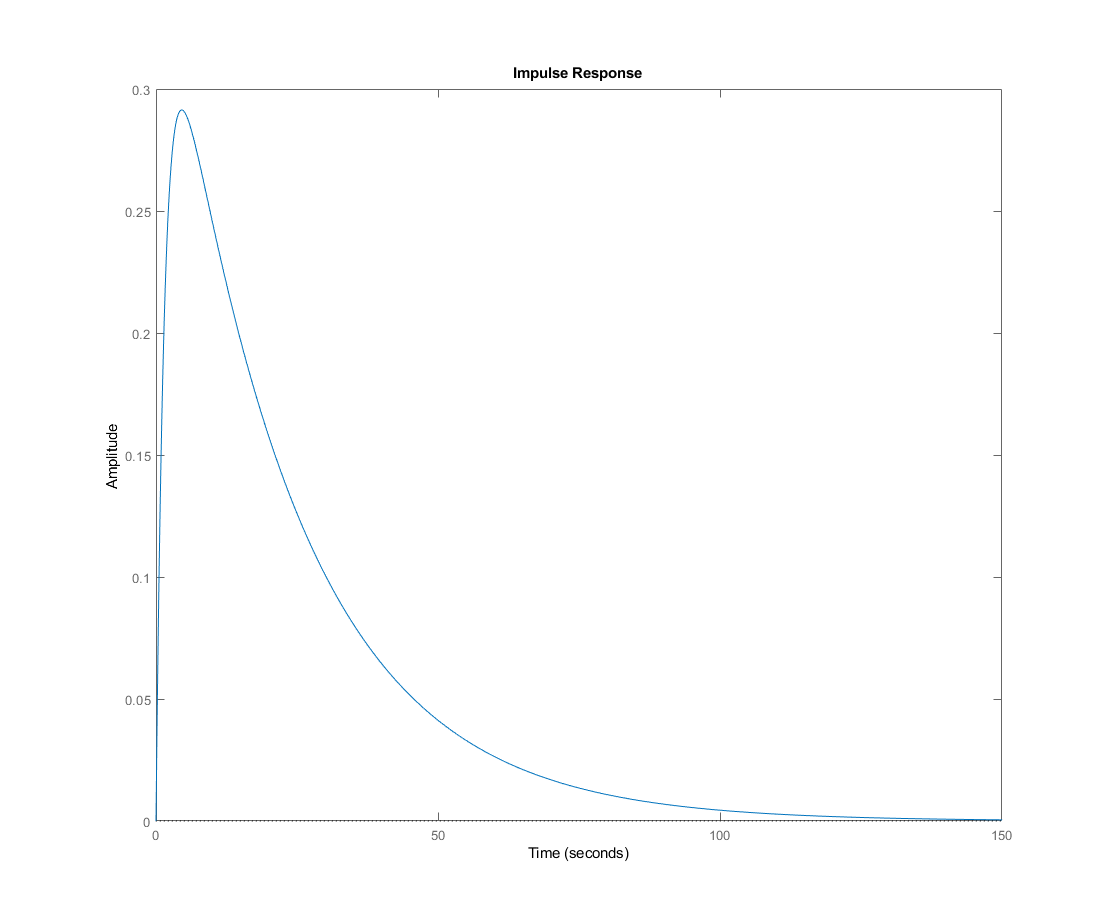
\includegraphics[width=15cm]{osc_impulse.png}
	\end{center}
\end{itemize}

\section{Zadanie 3 \textit{\small Wyznaczanie parametrów członów dynamicznych}}\label{sec:zad3}

\begin{itemize}
	\item Człon proporcjonalny
		
		Charakterystyka skokowa w dziedzinie czasu opisana jest wzorem:
		
		\begin{equation}
		h(t) = k * 1(t)
		\end{equation}
		
		Na wykresie widać, że niezależnie od czasu wykres przyjmuje wartość 8. Z tego wynika k = 8.
		
		Taka sama stała została wykorzystana do wyrysowania wykresów.
		
	\item Człon całkujący
	
	\begin{itemize}
		\item Charakterystyka skokowa
		
	Charakterystyka skokowa w dziedzinie czasu opisana jest wzorem:
	
\begin{equation}
h(t) = k * t
\end{equation}

Na wykresie widać że wartośc funkcji w 10 sekundzie wynosi 80:

\begin{equation}
h(10) = 80
\end{equation}

Z tego wynika k = 8

\item Charakterystyka impulsowa

Charakterystyka impulsowa w dziedzinie czasu opisana jest wzorem:

\begin{equation}
g(t) = k * 1(t)
\end{equation}

Z wykresu odczytujemy że niezależnie od czasu wartość funkcji wynosi 8, zatem k = 8.

Wyniki z odczytu wykresów obu tych charakterystyk są równe.

\end{itemize}
\end{itemize}

\end{document}